\documentclass[a5paper, 10pt]{article}

% Текст
\usepackage[utf8]{inputenc} % UTF-8 кодировка
\usepackage[russian]{babel} % Русский язык
\usepackage{indentfirst} % красная строка в первом параграфе в главе
% Отображение страниц
\usepackage{geometry} % размеры листа и отступов
\geometry{
	left=12mm,
	top=25mm,
	right=15mm,
	bottom=17mm,
	marginparsep=0mm,
	marginparwidth=0mm,
	headheight=10mm,
	headsep=7mm,
	nofoot}
\usepackage{afterpage,fancyhdr} % настройка колонтитулов
\pagestyle{fancy}
\fancypagestyle{style}{ % создание нового стиля style
	\fancyhf{} % очистка колонтитулов
	\fancyhead[LO, RE]{Индивидуальное домашнее задание №1} % название документа наверху
	%\fancyhead[RO, LE]{\leftmark} % название section наверху
	\fancyfoot[RO, LE]{\thepage} % номер страницы справа внизу на нечетных и слева внизу на четных
	\renewcommand{\headrulewidth}{0.25pt} % толщина линии сверху
	\renewcommand{\footrulewidth}{0pt} % толцина линии снизу
}
\fancypagestyle{plain}{ % создание нового стиля plain -- полностью пустого
	\fancyhf{}
	\renewcommand{\headrulewidth}{0pt}
}
\fancypagestyle{title}{ % создание нового стиля title -- для титульной страницы
	\fancyhf{}
	\fancyhead[C]{{\footnotesize
			Министерство образования и науки Российской Федерации\\
			Федеральное государственное автономное образовательное учреждение высшего образования
	}}
	\fancyfoot[C]{{\large 
			Санкт-Петербург, 2023-2024
	}}
	\renewcommand{\headrulewidth}{0pt}
}
\usepackage{comment}
% Математика
\usepackage{epigraph}
\usepackage{cancel}
\usepackage{amsmath, amsfonts, amssymb, amsthm} % Набор пакетов для математических текстов
%\usepackage{dmvnbase} % мехматовский пакет latex-сокращений
\usepackage{cancel} % зачеркивание для сокращений
% Рисунки и фигуры
\usepackage[pdftex]{graphicx} % вставка рисунков
\usepackage{wrapfig, subcaption} % вставка фигур, обтекая текст
\usepackage{caption} % для настройки подписей
\captionsetup{figurewithin=none,labelsep=period, font={small,it}} % настройка подписей к рисункам
% Рисование
\usepackage{tikz} % рисование
\usepackage{circuitikz}
\usepackage{pgfplots} % графики
% Таблицы
\usepackage{multirow} % объединение строк
\usepackage{multicol} % объединение столбцов
% Остальное
\usepackage[unicode, pdftex]{hyperref} % гиперссылки
\usepackage{enumitem} % нормальное оформление списков
\setlist{itemsep=0.15cm,topsep=0.15cm,parsep=1pt} % настройки списков
% Теоремы, леммы, определения...
\theoremstyle{definition}
\newtheorem{Def}{Определение}
\newtheorem*{Axiom}{Аксиома}
\theoremstyle{plain}
\newtheorem{Th}{Теорема}
\newtheorem{Lem}{Лемма}
\newtheorem{Cor}{Следствие}
\newtheorem{Ex}{Пример}
\theoremstyle{remark}
\newtheorem*{Note}{Замечание}
\newtheorem*{Solution}{Решение}
\newtheorem*{Proof}{Доказательство}
% Свои команды
\newcommand{\comb}[1]{\left[\hspace{-4pt}\begin{array}{l}#1\end{array}\right.\hspace{-5pt} } % совокупность уравнений
% Титульный лист
\usepackage{csvsimple-l3}
\newcommand*{\titlePage}{
	\thispagestyle{title}
	\begingroup
	\begin{center}
		%		{\footnotesize
			%			Министерство образования и науки Российской Федерации\\
			%			Федеральное государственное автономное образовательное учреждение высшего образования
			%		}
		%		
		\vspace*{6ex}
		
		{\small
			САНКТ-ПЕТЕРБУРГСКИЙ НАЦИОНАЛЬНЫЙ ИССЛЕДОВАТЕЛЬСКИЙ УНИВЕРСИТЕТ ИТМО	
		}
		
		\vspace*{2ex}
		
		{\normalsize
			Факультет систем управления и робототехники
		}
		
		\vspace*{15ex}
		
		{\Large \bfseries 
			Индивидуальное домашнее задание №1
		}
\vspace*{3ex}
		
		{ \Large 
			Вариант 3
		}
\vspace*{3ex}
		
		{  \bfseries 
			по дисциплине Дифференциальные уравнения
		}
	\end{center}
	\vspace*{20ex}
	\begin{flushright}
		{\large 
			\underline{Выполнила}: студентка гр. \textbf{R3238}\\
			\begin{flushright}
				\textbf{Нечаева А. А.}\\
			\end{flushright}
		}
		
		\vspace*{5ex}
		
		{\large 
			\underline{Преподаватель}: \textit{Бойцев Антон Александрович}
		}
	\end{flushright}	
	\newpage
	\setcounter{page}{1}
	\endgroup}

\begin{document}
	\titlePage
	\pagestyle{style}
	
\newpage
\epigraph{Трудность решения в какой-то мере входит в само понятие задачи: там, где нет трудности, нет и задачи.}{Д. Пойа}

\section{}
Привести заменой $x=z^m$ уравнение 
\begin{equation*}
(xy^2+1)yx' + 2x = 0, \, x > 0, \, y > 0
\end{equation*}
к однородному и решить его. Записать ответ в виде $F(x, y) = C$.\\
\\
\textit{\textbf{Решение:}}\\
Пусть $x=z^m, \, y = z$, тогда $x'=mz'z^{m-1}$, запишем получившееся уравнение:
\begin{equation*}
(z^mz^2+1)zmz'z^{m-1} + 2z^m = 0, \, z^m > 0, \, z > 0
\end{equation*}
\begin{equation*}
mz'z^{2m+2}+mz'z^{m} + 2z^m = 0
\end{equation*}
\begin{equation*}
mz'z^{2m+2}= -(mz' + 2)z^m
\end{equation*}
\begin{equation*}
2m+2 = m \to m = -2
\end{equation*}
Таким образом, $x = z^{-2}, \, x' = -2z' z^{-3}$, подставим в исходное уравнение, получим:
\begin{equation*}
-2z' z^{-3}( z^{-2}y^2+1)y + 2 z^{-2} = 0 \, \left| \right. : -2z^{-2} \neq 0
\end{equation*}
\begin{equation*}
z' z^{-1}( z^{-2}y^2+1)y -1 = 0 
\end{equation*}
\begin{equation*}
z' z^{-3}y^3+ z' z^{-1}y -1 = 0 
\end{equation*}
Полученное уравнение является однородным, убедимся, подставив $z = \lambda z, \, y = \lambda y$:
\begin{equation*}
 F( \lambda z,\, \lambda y ) = z' \lambda^{-3} z^{-3} \lambda^3y^3+ z' \lambda^{-1}z^{-1} \lambda y -1 =  \lambda^0  F(  z,\,  y )
\end{equation*}
Решаем уравнение:
\begin{equation*}
z'  z^{-1}y(z^{-2}y^2+ 1) -1 = 0 
\end{equation*}
Подстановка: $z = ty, \, z' = t'y + t$
\begin{equation*}
(t'y + t)  (ty)^{-1}y((ty)^{-2}y^2+ 1) -1 = 0 
\end{equation*}
\begin{equation*}
(t'y + t) t^{-1}(t^{-2}+ 1) -1 = 0 
\end{equation*}
\begin{equation*}
t'y + t= \frac{t}{t^{-2}+ 1}, \, \, t^{-2}+ 1 \neq 0 \, (\textit{из условия всегда выполнено})
\end{equation*}
\begin{equation*}
t'y = \frac{t}{t^{-2}+ 1} - t
\end{equation*}
\begin{equation*}
\frac{dt}{dy}y = \frac{t}{t^{-2}+ 1} - t
\end{equation*}
\begin{equation*}
\frac{dt}{dy}y = \frac{t - t^{-1}- t }{t^{-2}+ 1} 
\end{equation*}
\begin{equation*}
\frac{dt}{dy}y = \frac{- t^{-1}}{t^{-2}+ 1} 
\end{equation*}
\begin{equation*}
-t(t^{-2}+ 1) \, dt  = \frac{dy}{y}
\end{equation*}
\begin{equation*}
- \int (t^{-1} + t) \, dt  = \int \frac{dy}{y}
\end{equation*}
\begin{equation*}
- \ln t - \frac{t^2}{2}  = \ln y + C
\end{equation*}
\begin{equation*}
- \ln \frac{z}{y} - \frac{z^2}{2y^2}  = \ln y + C
\end{equation*}
\begin{equation*}
- \ln z +  \ln y - \frac{z^2}{2y^2}  = \ln y + C
\end{equation*}

\begin{equation*}
- \ln z  - \frac{z^2}{2y^2}  =  C
\end{equation*}
Обратная замена: $x = z^{-2} \to z = \frac{1}{\sqrt{x}}$
\begin{equation*}
- \ln \frac{1}{\sqrt{x}}   - \frac{1}{2xy^2}  =  C
\end{equation*}
\begin{equation*}
 \ln \sqrt{x}   - \frac{1}{2xy^2}  =  C
\end{equation*}

\textit{\textbf{Ответ:}} $\ln \sqrt{x}   - \frac{1}{2xy^2}  =  C$



\newpage
\section{}
Решить линейное уравнение методом вариации произвольных постоянных (методом Лагранжа). Пользуясь формулой общего решения линейного уравнения, проверьте полученный ответ.\\
Записать ответ в виде $y = f(x, C).$
\begin{equation*}
y' = \frac{2y}{x \ln x} + \frac{1}{x}, \, x > 1\\
\end{equation*}
\textit{\textbf{Решение:}}\\
Решим уравнение:
\begin{equation*}
y' = \frac{2y}{x \ln x}, \, x > 1\\
\end{equation*}
\begin{equation*}
\frac{dy}{dx} = \frac{2y}{x \ln x}, \, x > 1\\
\end{equation*}
\begin{equation*}
\frac{dy}{2y} = \frac{dx}{x \ln x}, \, \, y \neq 0
\end{equation*}
Заметим, что $y = 0$ также является решение уравнения $y' = \frac{2y}{x \ln x}$.
\begin{equation*}
 \int \frac{dy}{2y} = \int \frac{dx}{x \ln x}
\end{equation*}
\begin{equation*}
  \frac{1}{2} \ln |y| = \int \frac{d \ln x}{\ln x}
\end{equation*}
\begin{equation*}
  \frac{1}{2} \ln |y| = \ln \ln x + \ln C
\end{equation*}
\begin{equation*}
  \ln |y| =2 \ln C \ln x
\end{equation*}
\begin{equation*}
  y = C e^{ \ln ^2 x}
\end{equation*}
\begin{equation*}
  y = C  \ln ^2 x
\end{equation*}
Метод вариации произвольной постоянной -- примим $C = C(x)$ и подставим в исходное уравнение:
\begin{equation*}
C' \ln ^2 x + 2C \ln x \frac{1}{x}= \frac{2 C  \ln ^2 x}{x \ln x} + \frac{1}{x}
\end{equation*}
\begin{equation*}
C' \ln ^2 x =  \frac{1}{x}
\end{equation*}
\begin{equation*}
\int dC  = \int \ln ^{-2} x  \,\frac{dx}{x} 
\end{equation*}
\begin{equation*}
\int dC  = \int \ln ^{-2} x \, d \ln x
\end{equation*}
\begin{equation*}
C  =  - \ln ^{-1} x + A, \, A = const
\end{equation*}
В итоге получим:
\begin{equation*}
  y = (A - \ln ^{-1} x  )  \ln ^2 x, \, A = const
\end{equation*}
\begin{equation*}
  y = A\ln ^2 x - \ln x , \, A = const
\end{equation*}
Проверим полученный результат, возпользовавшись формулой общего решения линейного уравнения:
\begin{equation*}
  y = \left( A + \int q(x) e^{\int p(x) dx} dx \right) e^{-\int p(x) dx}
\end{equation*}
\begin{equation*}
  y = \left( A + \int \frac{1}{x} e^{-\int \frac{2}{x \ln x} dx} dx \right) e^{\int \frac{2}{x \ln x}  dx}
\end{equation*}
\begin{equation*}
  y = \left( A + \int \frac{1}{x} e^{-2\ln \ln x + B} dx \right) e^{2\ln \ln x + B}, \, \, B =const
\end{equation*}
\begin{equation*}
  y = \left( A + \int \frac{1}{x B \ln ^2 x} dx \right)B \ln ^2 x 
\end{equation*}
\begin{equation*}
  y = \left( A  - \frac{1}{ B \ln x} \right)B \ln ^2 x 
\end{equation*}

\begin{equation*}
  y = AB  \ln ^2 x   - \ln x
\end{equation*}
\\
\textit{\textbf{Ответ:}} $  y = A\ln ^2 x - \ln x , \, A = const$

\newpage
\section{}
Привести уравнение Риккати к линейному. Решить полученное линейное уравнение, используя метод интегрирующего множителя.\\
Записать ответ в виде $F(x, y) = C$.
\begin{equation*}
xy' = x^3 + (1 - 2x^2)y + xy^2
\end{equation*}
\textit{\textbf{Решение:}}\\
Найдем частное решение вида $y = Cx$:
\begin{equation*}
x \left(  Cx \right)' = x^3 + (1 - 2x^2) Cx + x\left(  Cx \right)^2
\end{equation*}
\begin{equation*}
x C = x^3 + (1 - 2x^2) Cx + x^3C^2
\end{equation*}
\begin{equation*}
x C = x^3 + Cx - 2Cx^3 + x^3C^2
\end{equation*}
\begin{equation*}
x^3 - 2Cx^3 + x^3C^2 = 0
\end{equation*}
\begin{equation*}
1 - 2C + C^2 = 0,  \, \, x \neq 0
\end{equation*}
\begin{equation*}
\left(1 - C \right)^2 = 0 \to C = 1
\end{equation*}
Частное решение  $y = x$, замена $y = x + z$:
\begin{equation*}
x(z' + 1) = x^3 + (1 - 2x^2)(x + z) + x(x + z)^2
\end{equation*}
\begin{equation*}
xz' + x = x^3 + x - 2x^3 + z - 2zx^2 + x^3 +2zx^2 +x z^2
\end{equation*}
\begin{equation*}
xz'  =  z +x z^2 \, \left| \right. : x \neq 0
\end{equation*}

\textit{Заметим, что x = 0 не является решением уравнения, т.к. не обращает его в тождество}.
\begin{equation*}
z'  =  \frac{z}{x} + z^2 
\end{equation*} 
Получено уравнение Бернулли вида $y' = q(x)y + p(x) y^n$.
\begin{equation*}
z'  =  \frac{z}{x} + z^2  \, \left| \right. :  z^2 \neq 0 
\end{equation*} 
Заметим, что $z = 0$ -- тоже решение.
\begin{equation*}
 \frac{z'}{ z^2}  =  \frac{1}{zx} + 1 
\end{equation*} 
Замена: $t = \frac{1}{z}$ и $t' = - \frac{z'}{z^2}$:
\begin{equation*}
-t'  =  \frac{t}{x} + 1 
\end{equation*} 
Получено линейное уравнение. Решим его методом интегрирующего множителя:
\begin{equation*}
\left(   \frac{t}{x} + 1  \right) dx + dt = 0
\end{equation*}
\begin{equation*}
P =  \frac{t}{x} + 1
\end{equation*}
\begin{equation*}
Q = 1
\end{equation*}
\begin{equation*}
\left( \mu P \right)'_t = \left( \mu Q \right)'_x
\end{equation*}
\begin{equation*}
 \mu'_t P + \mu P'_t = \mu'_x Q  +  \mu Q'_x
\end{equation*}
\begin{equation*}
 \mu'_t  \left(   \frac{t}{x} + 1  \right) +  \frac{\mu}{x} = \mu'_x 
\end{equation*}
Пусть $\mu = \mu(x)$, тогда $\mu'_t = 0$:
\begin{equation*}
 \frac{\mu}{x} = \mu'_x  \, \left| \right. :  \mu \neq 0 
\end{equation*}
\begin{equation*}
 \int \frac{dx}{ x}  = \int \frac{d\mu}{\mu} 
\end{equation*} 
\begin{equation*}
 \ln |x|  = \ln |\mu| + C 
\end{equation*} 
Интегрирующий множитель: $\mu = x$:
\begin{equation*}
x \left(   \frac{t}{x} + 1  \right) dx + x dt = 0
\end{equation*}
\begin{equation*}
\left(  t + x \right) dx + x dt = 0
\end{equation*}
Получено уравнение в полных дифференциалах вида:
\begin{equation*}
\frac{\partial F}{\partial x}dx + \frac{\partial F}{\partial t}dt = 0
\end{equation*}

\begin{equation*}
\frac{\partial F}{\partial t} = x
\end{equation*}
\begin{equation*}
\int \partial F = \int x \partial t \, \, \to \, \, F = xt + C(x)
\end{equation*}
\begin{equation*}
\frac{\partial F}{\partial x} = t + C' =  t + x  \, \, \to \, \, C = \frac{x^2}{2} + A, \, A = const
\end{equation*}
В итоге получаем:
\begin{equation*}
F =  xt +  \frac{x^2}{2} + A
\end{equation*}
Обратная замена $t = \frac{1}{z}$:
\begin{equation*}
F =   \frac{x}{z} +  \frac{x^2}{2} + A
\end{equation*}
И $ z = y - x$:
\begin{equation*}
F =   \frac{x}{y - x} +  \frac{x^2}{2} + A
\end{equation*}

\textit{\textbf{Ответ:}} $ \frac{x}{y - x} +  \frac{x^2}{2}  = -A, \, A = const$  , $ y =   0$ и $y = x$ -- тоже решения.
\begin{comment}
Получено линейное уравнение. Решим его методом вариации произвольной постоянной:
\begin{equation*}
t'  =  -\frac{t}{x}
\end{equation*} 
\begin{equation*}
 \frac{dt}{dx}  = - \frac{t}{x} \, \left| \right. :  t \neq 0 
\end{equation*} 
\begin{equation*}
 \frac{dt}{t}  = - \frac{dx}{x} 
\end{equation*} 
Заметим, что $t = 0$ -- тоже решение.
\begin{equation*}
 \int \frac{dt}{t}  =   -  \int \frac{dx}{x} 
\end{equation*} 
\begin{equation*} 
 \ln |t|  =   -  \ln |x| + \ln C
\end{equation*} 
\begin{equation*} 
 \ln |t|  =   -  \ln Cx
\end{equation*} 
\begin{equation*} 
 \ln |t|  = \ln \frac{C }{x}
\end{equation*} 
\begin{equation*} 
 t =  \frac{C }{x}
\end{equation*} 
Заметим, что $t = 0$ -- решение при $C = 0$.\\
Пусть $C = C(x)$:
\begin{equation*}
t'  = -\frac{t}{x} - 1 
\end{equation*} 
\begin{equation*}
\left(  \frac{C}{x} \right)'  = - \frac{C}{x^2} - 1 
\end{equation*}
\begin{equation*}
  \frac{C' x - C }{x^2}   =  - \frac{C}{x^2} - 1
\end{equation*}
\begin{equation*}
  \frac{C'}{x}   =   - 1 
\end{equation*}
\begin{equation*}
 \int dC   =   -\int xdx 
\end{equation*}
\begin{equation*}
  C  =   - \frac{x^2}{2} + A, \, \, A = const
\end{equation*}

Запишем теперь:
\begin{equation*} 
 t =  \frac{A -  \frac{x^2}{2}}{x} =  \frac{  A}{x} -  \frac{ x}{2} , \, \, A = const
\end{equation*} 
Обратная замена $ z = \frac{1}{t}$:
\begin{equation*} 
 z =  \frac{2x}{2A - x^2} , \, \, A = const
\end{equation*} 
\begin{equation*} 
 y =   x +  \frac{2x}{2A - x^2} , \, \,  A = const
\end{equation*} 
и еще одно решение:
\begin{equation*} 
 y =   0
\end{equation*} 

\textit{\textbf{Ответ:}} $ y =   x + \frac{2x}{2A - x^2}, \, A = const$ , $ y =   0$ и $y = x$ -- тоже решения.
\end{comment}

\newpage
\section{}
Решить уравнение в дифференциалах, подобрав интегрирующий множитель в виде $\mu (x, y) = (x+y^2)^{\alpha}$.\\
Записать ответ в виде $F(x, y) = C$.
\begin{equation*}
2y(x + y^2 - 1) dy + (x^2y^2+x^3 - 1)dx = 0
\end{equation*}
\textit{\textbf{Решение:}}\\
\begin{equation*}
P = 2y(x + y^2 - 1) 
\end{equation*}
\begin{equation*}
Q = x^2y^2+x^3 - 1
\end{equation*}
\begin{equation*}
\left( \mu P \right)'_x = \left( \mu Q \right)'_y
\end{equation*}
\begin{equation*}
 \mu'_x P + \mu P'_x = \mu'_y Q  +  \mu Q'_y
\end{equation*}
\begin{equation*}
 \mu'_y =  \left(  (x+y^2)^{\alpha} \right)'_y  = 2y{\alpha} (x+y^2)^{\alpha - 1}
\end{equation*}
\begin{equation*}
 \mu'_x =  \left(  (x+y^2)^{\alpha} \right)'_x  = {\alpha} (x+y^2)^{\alpha - 1}
\end{equation*}
\begin{equation*}
 P'_x =  \left(  2y(x + y^2 - 1)  \right)'_x = 2y
\end{equation*}
\begin{equation*}
 Q'_y=  \left(  x^2y^2+x^3 - 1  \right)'_y = 2yx^2
\end{equation*}
\begin{equation*}
  {\alpha} (x+y^2)^{\alpha - 1}  2y(x + y^2 - 1) + 2y(x+y^2)^{\alpha}  = 2y{\alpha} (x+y^2)^{\alpha - 1} ( x^2y^2+x^3 - 1)  +  (x+y^2)^{\alpha}  2yx^2
\end{equation*}
\begin{equation*}
 \bcancel{ 2y (x+y^2)^{\alpha - 1}} ( {\alpha}(x + y^2 - 1) +(x+y^2)) =  \bcancel{ 2y (x+y^2)^{\alpha - 1}}({\alpha} ( x^2y^2+x^3 - 1)  +  (x+y^2)x^2)
\end{equation*}
\begin{equation*}
  {\alpha}(x + y^2 - 1) +x+y^2 =  {\alpha} ( x^2y^2+x^3 - 1)  +  x^3+y^2x^2
\end{equation*}
\begin{equation*}
  {\alpha}(x + y^2 - 1 - x^2y^2-x^3 + 1) =    x^3+y^2x^2 -x-y^2 
\end{equation*}
\begin{equation*}
  {\alpha}(x + y^2  - x^2y^2-x^3 ) =    x^3+y^2x^2 -x-y^2 
\end{equation*}
\begin{equation*}
  {\alpha} = -1
\end{equation*}
Полученный интегральный множитель: $\mu = \frac{1}{x+y^2}$:
\begin{equation*}
2y\frac{x + y^2 - 1}{x+y^2}dy + \frac{x^2y^2+x^3 - 1}{x+y^2} dx = 0
\end{equation*}
Получено уравнение в полных дифференциалах вида:
\begin{equation*}
\frac{\partial F}{\partial y}dy + \frac{\partial F}{\partial x}dx = 0
\end{equation*}

\begin{multline*}
F = \int \frac{x^2y^2+x^3 - 1}{x+y^2} dx = \int \frac{x^2(y^2+x) - 1}{x+y^2} dx = \int x^2 dx - \int \frac{1}{x+y^2} dx =\\
= \frac{x^3}{3} - \ln |x + y^2| + C
\end{multline*}
Пусть $C = C(y)$:
\begin{equation*}
\frac{\partial F}{\partial y} = -\frac{2y}{x + y^2} + C'_y
\end{equation*}
\begin{equation*}
2y\frac{x + y^2 - 1}{x+y^2} =  -\frac{2y}{x + y^2} + C'_y
\end{equation*}
\begin{equation*}
2y - \frac{ 2y}{x+y^2} =  -\frac{2y}{x + y^2} + C'_y
\end{equation*}
\begin{equation*}
  C'_y = 2y
\end{equation*}
\begin{equation*}
\int  dC= \int 2ydy
\end{equation*}
\begin{equation*}
  C = y^2 + A, \, \, A = const
\end{equation*}

\begin{equation*}
F = \frac{x^3}{3} - \ln |x + y^2| +  y^2 + A, \, \, A = const
\end{equation*}

\textit{\textbf{Ответ:}} $F = \frac{x^3}{3} - \ln |x + y^2| +  y^2 + A, \, \, A = const$









\newpage
\section{}
Решить уравнение методом введения параметра. \\
Записать ответ в виде $x = f(y, C)$.\\
Исследовать на наличие особых решений. Построить на одной координатной плоскости графики нескольких интегральных кривых и, при наличии, особых решений.
\begin{equation*}
2x = \frac{y}{y'} + \ln (yy'), \, y >0\\
\end{equation*}
\textit{\textbf{Решение:}}\\
Введем параметр $p = y'$, сразу запишем $p = \frac{dy}{dx}, \, \, dy = pdx, \, \, dx = \frac{dy}{p}$:
\begin{equation*}
2x = \frac{y}{p} + \ln (yp)
\end{equation*}
Продифференцируем полученное выражение:
\begin{equation*}
2dx = d\frac{y}{p} + d\ln (yp)
\end{equation*}
\begin{equation*}
2dx = \frac{pdy - ydp}{p^2} + \frac{pdy + ydp}{yp}
\end{equation*}
\begin{equation*}
2\frac{dy}{p} = \frac{pdy - ydp}{p^2} + \frac{pdy + ydp}{yp}
\end{equation*}
\begin{equation*}
2dy = \frac{pdy - ydp}{p} + \frac{pdy + ydp}{y}
\end{equation*}
\begin{equation*}
2dy =dy - \frac{ydp}{p} + dp +\frac{pdy}{y}
\end{equation*}
Сгруппируем по дифференциалам:
\begin{equation*}
\left( 1 - \frac{p}{y} \right) dy = \left(1 - \frac{y}{p} \right) dp
\end{equation*}
Замена: $t = \frac{y}{p}, \, \, y = tp, \, \, dy = pdt + tdp$
\begin{equation*}
\left( 1 - \frac{1}{t} \right) ( pdt + tdp) = \left(1 - t \right) dp
\end{equation*}
\begin{equation*}
 pdt + tdp - \frac{ pdt}{t}  - dp = dp  - t dp
\end{equation*}
Сгруппируем по дифференциалам:
\begin{equation*}
 p \left(1  - \frac{ 1}{t} \right) dt  = 2 (1  - t) dp
\end{equation*}
Получено уравнение с разделяющимися переменными
\begin{equation*}
 p \left(1  - \frac{ 1}{t} \right) dt  = 2 (1  - t) dp \, \left| : p (1  - t) \neq 0 \right.
\end{equation*}
Заметим, что $p = 0$ не является решением.\\
Проверим $t = 1$:
\begin{equation*}
 t = 1 \, \to  \frac{y}{y'} = 1 \, \to y = y' \, \to y = B e^x, \, B = const
\end{equation*}
Подставим в исходное дифференциальное уравнение:
\begin{equation*}
2x = \frac{ B e^x}{ B e^x} + \ln ( B^2 e^x)
\end{equation*}
\begin{equation*}
2x = 1 + \ln B^2 + x
\end{equation*}
\begin{equation*}
x = 1 + \ln B^2
\end{equation*}
-- тоже решение.





\begin{equation*}
  \left(1  - \frac{ 1}{t} \right) \frac{1}{ (1  - t) } dt  =  \frac{2}{p} dp 
\end{equation*}
\begin{equation*}
 - \frac{1}{ t } dt  =  \frac{2}{p} dp 
\end{equation*}
\begin{equation*}
 - \int \frac{1}{ t } dt  = \int \frac{2}{p} dp 
\end{equation*}
\begin{equation*}
 - \ln | t| + C  = 2 \ln| p|
\end{equation*}
\begin{equation*}
 \ln \frac{C}{t}  =  \ln p^2
\end{equation*}
\begin{equation*}
  \frac{C}{t}  =   p^2
\end{equation*}
\begin{equation*}
  \frac{Cp}{y}  =   p^2
\end{equation*}
\begin{equation*}
  \frac{C}{y}  =   p
\end{equation*}

\begin{equation*}
 y   =   \frac{C}{p}
\end{equation*}
Теперь найдем $x(p)$:
\begin{equation*}
2x = \frac{y}{p} + \ln (yp)
\end{equation*}
\begin{equation*}
2x = \frac{ y}{ \frac{C}{y}} + \ln ( y  \frac{C}{y})
\end{equation*}
\begin{equation*}
2x = \frac{ y^2}{C} + \ln  C
\end{equation*}
\begin{equation*}
x = \frac{ y^2}{2C} +  \frac {\ln  C}{2}
\end{equation*}
Проверка на наличие особых решений.\\
Найдем $p-$дискриминантную кривую:
\begin{equation*}
F(x, y, y')= \frac{y}{y'}+\ln (yy') - 2x
\end{equation*}
\begin{equation*}
\frac{\partial F}{\partial y'} = - \frac{y}{y'^2} + \frac{1}{y'}  = 0 \, \, \to  1  =  \frac{y}{y'} \, \, \to y' = y
\end{equation*}
Подставим полученное выражение для $y'$ в исходное уравнение:
\begin{equation*}
2x = \frac{y}{y} + \ln (y^2) \, \, \to 2x = 1 + 2\ln (y) \, \, \to y = e^{x - 0.5}
\end{equation*}

Полученная кривая --  $p-$дискриминантную кривая.\\
Проверим, является ли она решением:
\begin{equation*}
2x = \frac{e^{x-0.5}}{e^{x- 0.5}} + \ln (e^{2x- 1}) \, \, \to 2x  = 1 + 2x - 1
\end{equation*}
$p-$дискриминантную кривая является решением исходного дифференциального уравнения.\\
Выразим дискриминантную кривую через $x$:
\begin{equation*}
 y = e^{x - 0.5} \, \, \to \, \,  x = \ln y + 0.5
\end{equation*}


\begin{equation*}
   \frac{ y_0^2}{2C} +  \frac {\ln  C}{2}  = \ln y_0 + 0.5 \, \, \to y_0 = \sqrt{ C}
\end{equation*}

\begin{equation*}
   \frac{ y_0}{C}   = \frac{1}{y_0} \, \, \to y_0^2 =  C
\end{equation*}
В каждой точке дискриминантной кривой её касается другая кривая семейства: $x = \frac{ y^2}{2C} +  \frac {\ln  C}{2}$, для которой $C=y^2$, значит, $x = \ln y + 0.5 $ является особым решением.\\




\begin{figure}[h]
\center{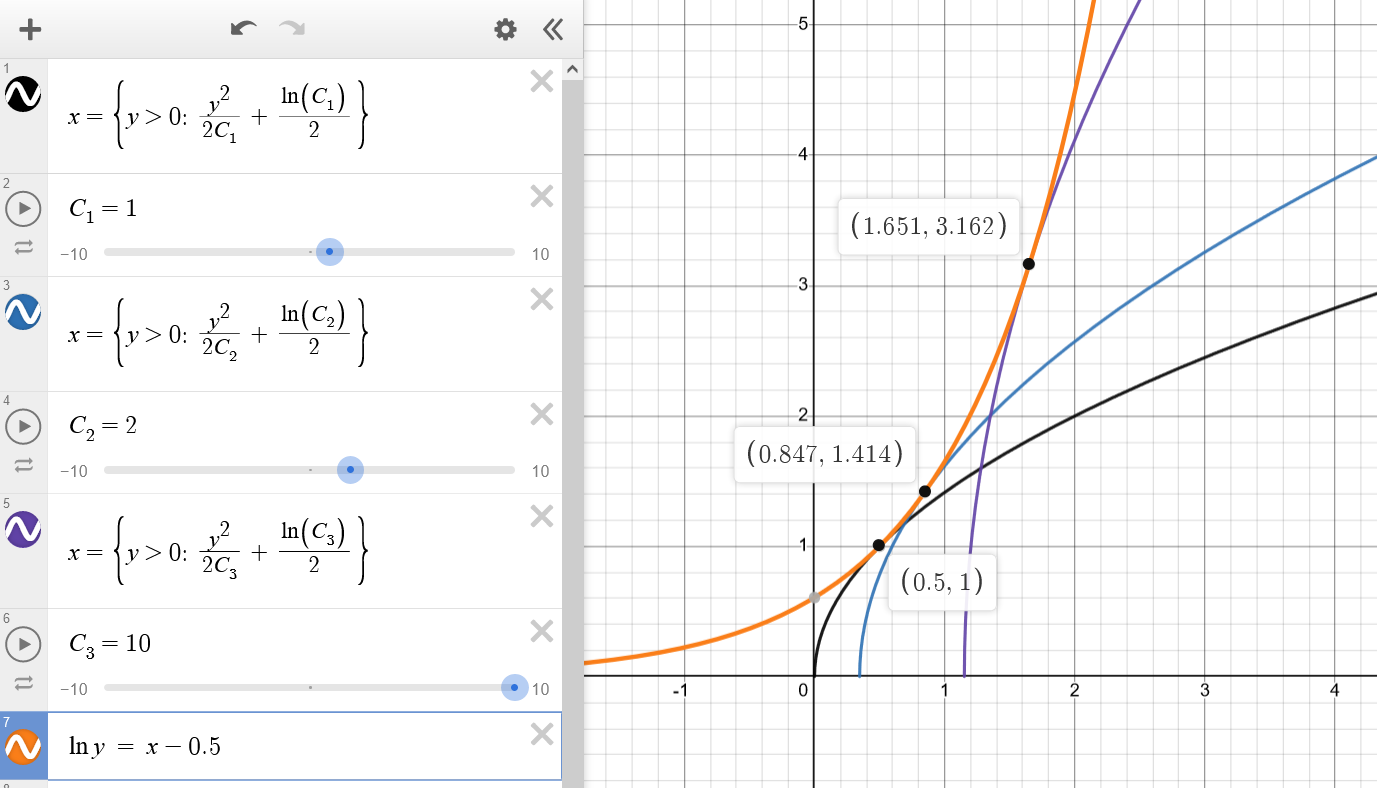
\includegraphics[width=1\linewidth]{int.png}}
\caption{Интегральные кривые и кривая особого решения (оранжевая)}
\end{figure}

\textit{\textbf{Ответ:}} $x = \frac{ y^2}{2C} +  \frac {\ln  C}{2}$,  $x = \ln y + 0.5 $ -- особое решение.

\end{document}













